\chapter{Ressources narratologiques}
\fancyhead[LO]{Ressources narratologiques}




% level size                     (5.3 Graph Geometry, see p. 84)
% parent distance in child graph (5.3 Graph Geometry, see p. 89)
% child  distance in child graph (5.3 Graph Geometry, see p. 87)
% edges=none                     (8.2 Edges Types, see p. 212)
% edges down by                  (8.8 Edge Shifting, see p. 233)
% edges up   by                  (8.8 Edge Shifting, see p. 233)
% union                          (4.4 Subgraph 'union', see p. 69)
% xshift tikz option             (2.5.3 Manual Position Adjustments, see p. 48)

\paragraph*{Généalogie de la famille royale}
\null{~}\vspace{1em}

\noindent\resizebox{\textwidth}{!}{%
  \begin{tikzpicture}
  \gtrset{edges={foreground={line width=0.03em,black},no background}}
  \genealogytree[template=signpost,
                 level size=0.6cm,
                 parent distance in child graph=0.5cm,
                 child  distance in child graph=0.5cm,
                 box={colback=white,no shadow,boxrule=0.03em,sharp corners}]{
    child[edges down by = 1 of 6]{% To put edges in the middle: 1/3 + 1/6 = 1/2
      p[tikz={xshift=1.2cm}]{\cleopatre}
      g[tikz={xshift=2cm}]{\roi}
      child{
        g{\ela}
        p[edges=none]{\catin}
        g{\elena}
        c{\cleopatre}
      }
      union[edges up by = 1 of 6]{% To put edges in the middle: 2/3 - 1/6 = 1/2
        p[tikz={xshift=2.5cm}]{\reine}
        c{\princesse}
        c{\vladimir}
      }
    }
  }
\end{tikzpicture}
}

\paragraph*{Structure spatio-sociale de l’Arche}
\null{~}\vspace{1em}

\begin{center}
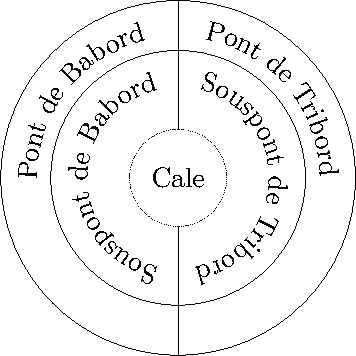
\includegraphics[width=0.6\textwidth]{structure-de-larche.pdf}
\end{center}



